  \subsection{Características de detección}

    El esquema de conexiones que se debe implementar con los dispositivos antes mencionados, se puede observar en
    la Figura~\ref{fig:EsquemaConexiones}.

    \begin{figure}[H]
      \centering
      \frame{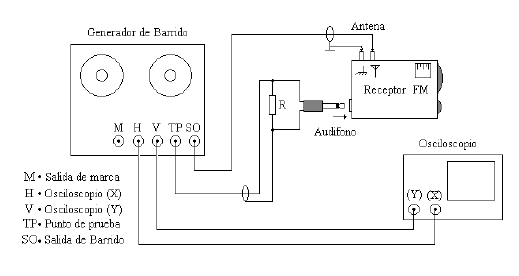
\includegraphics[width=0.6\textwidth]{Imagenes/ActividadPractica/CaracteristicasDeDeteccion/EsquemaConexiones.png}}
      \caption{Esquema de conexiones para las mediciones.}
      \label{fig:EsquemaConexiones}
    \end{figure}


    \begin{figure}[H]
      \centering
      \begin{subfigure}[ht]{0.48\textwidth}
        \frame{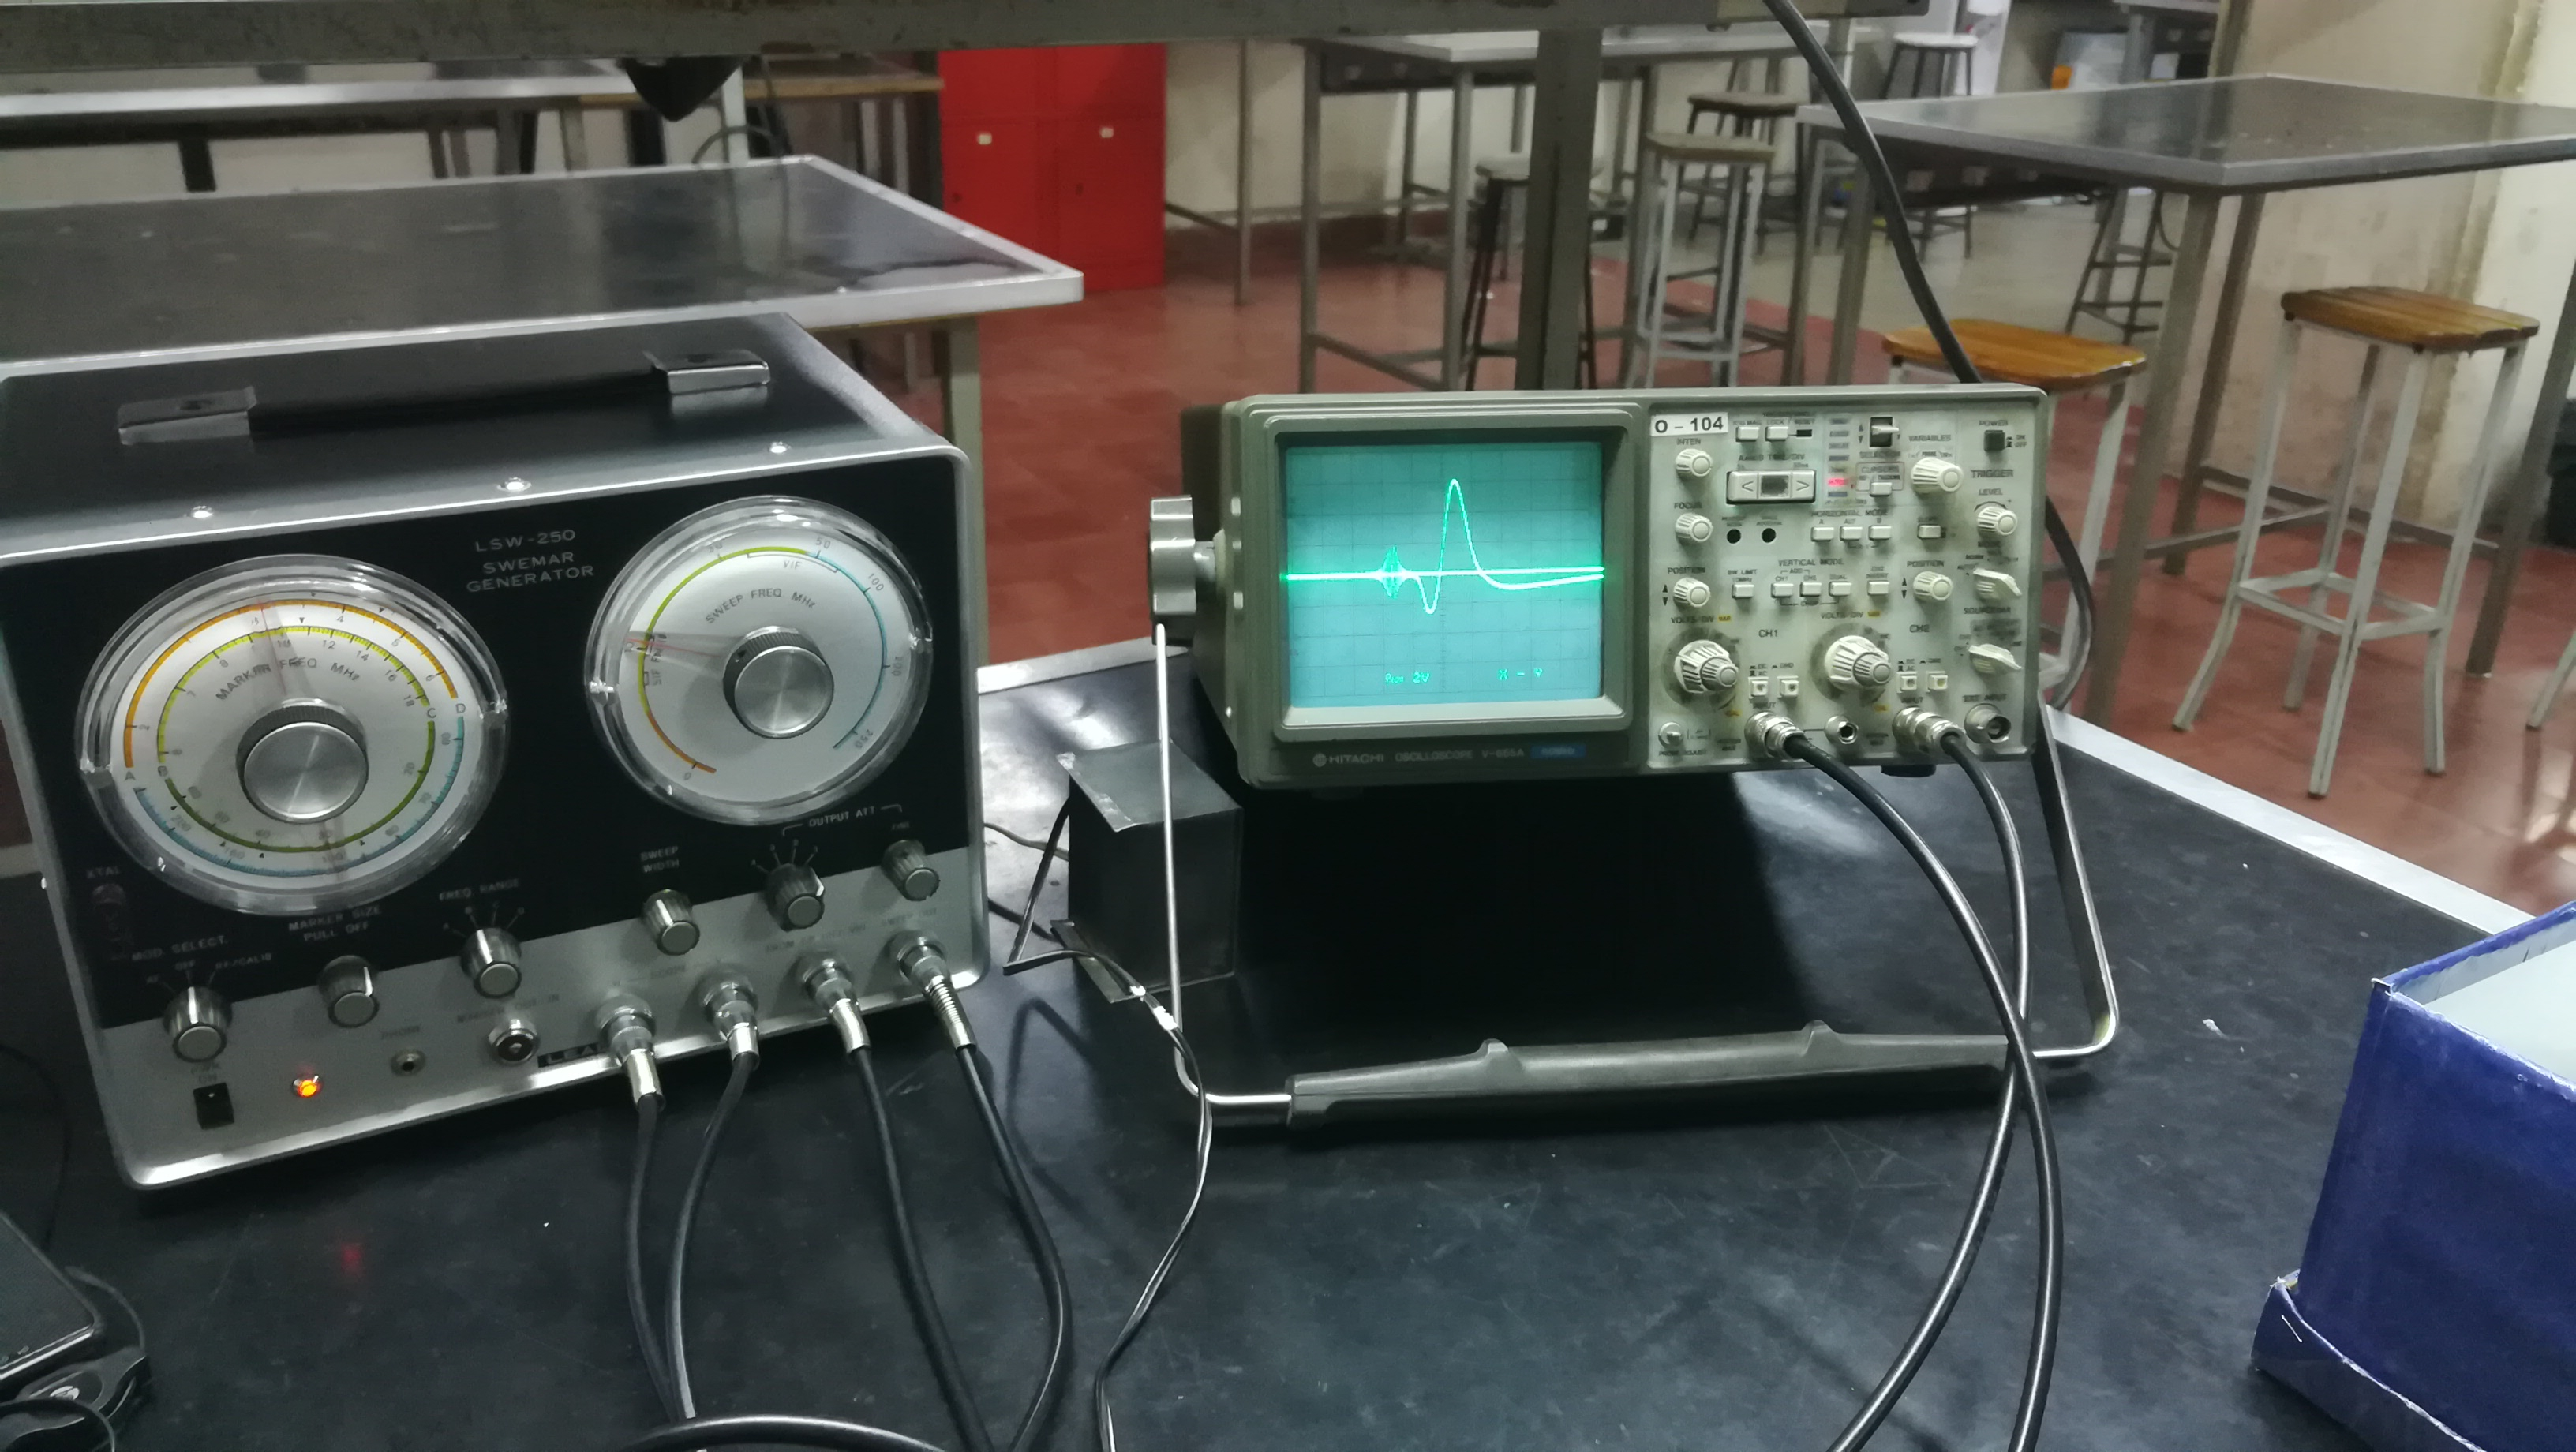
\includegraphics[width=\textwidth]{Imagenes/ActividadPractica/CaracteristicasDeDeteccion/Exp2.1_AmpliFI_InstrumentosConMarcaAIzquierda.jpg}}
        \caption{Disposición de instrumentos.}
        \label{fig:InstrumentosParaFI}
      \end{subfigure}
      \hfill 
      \begin{subfigure}[ht]{0.48\textwidth}
        \frame{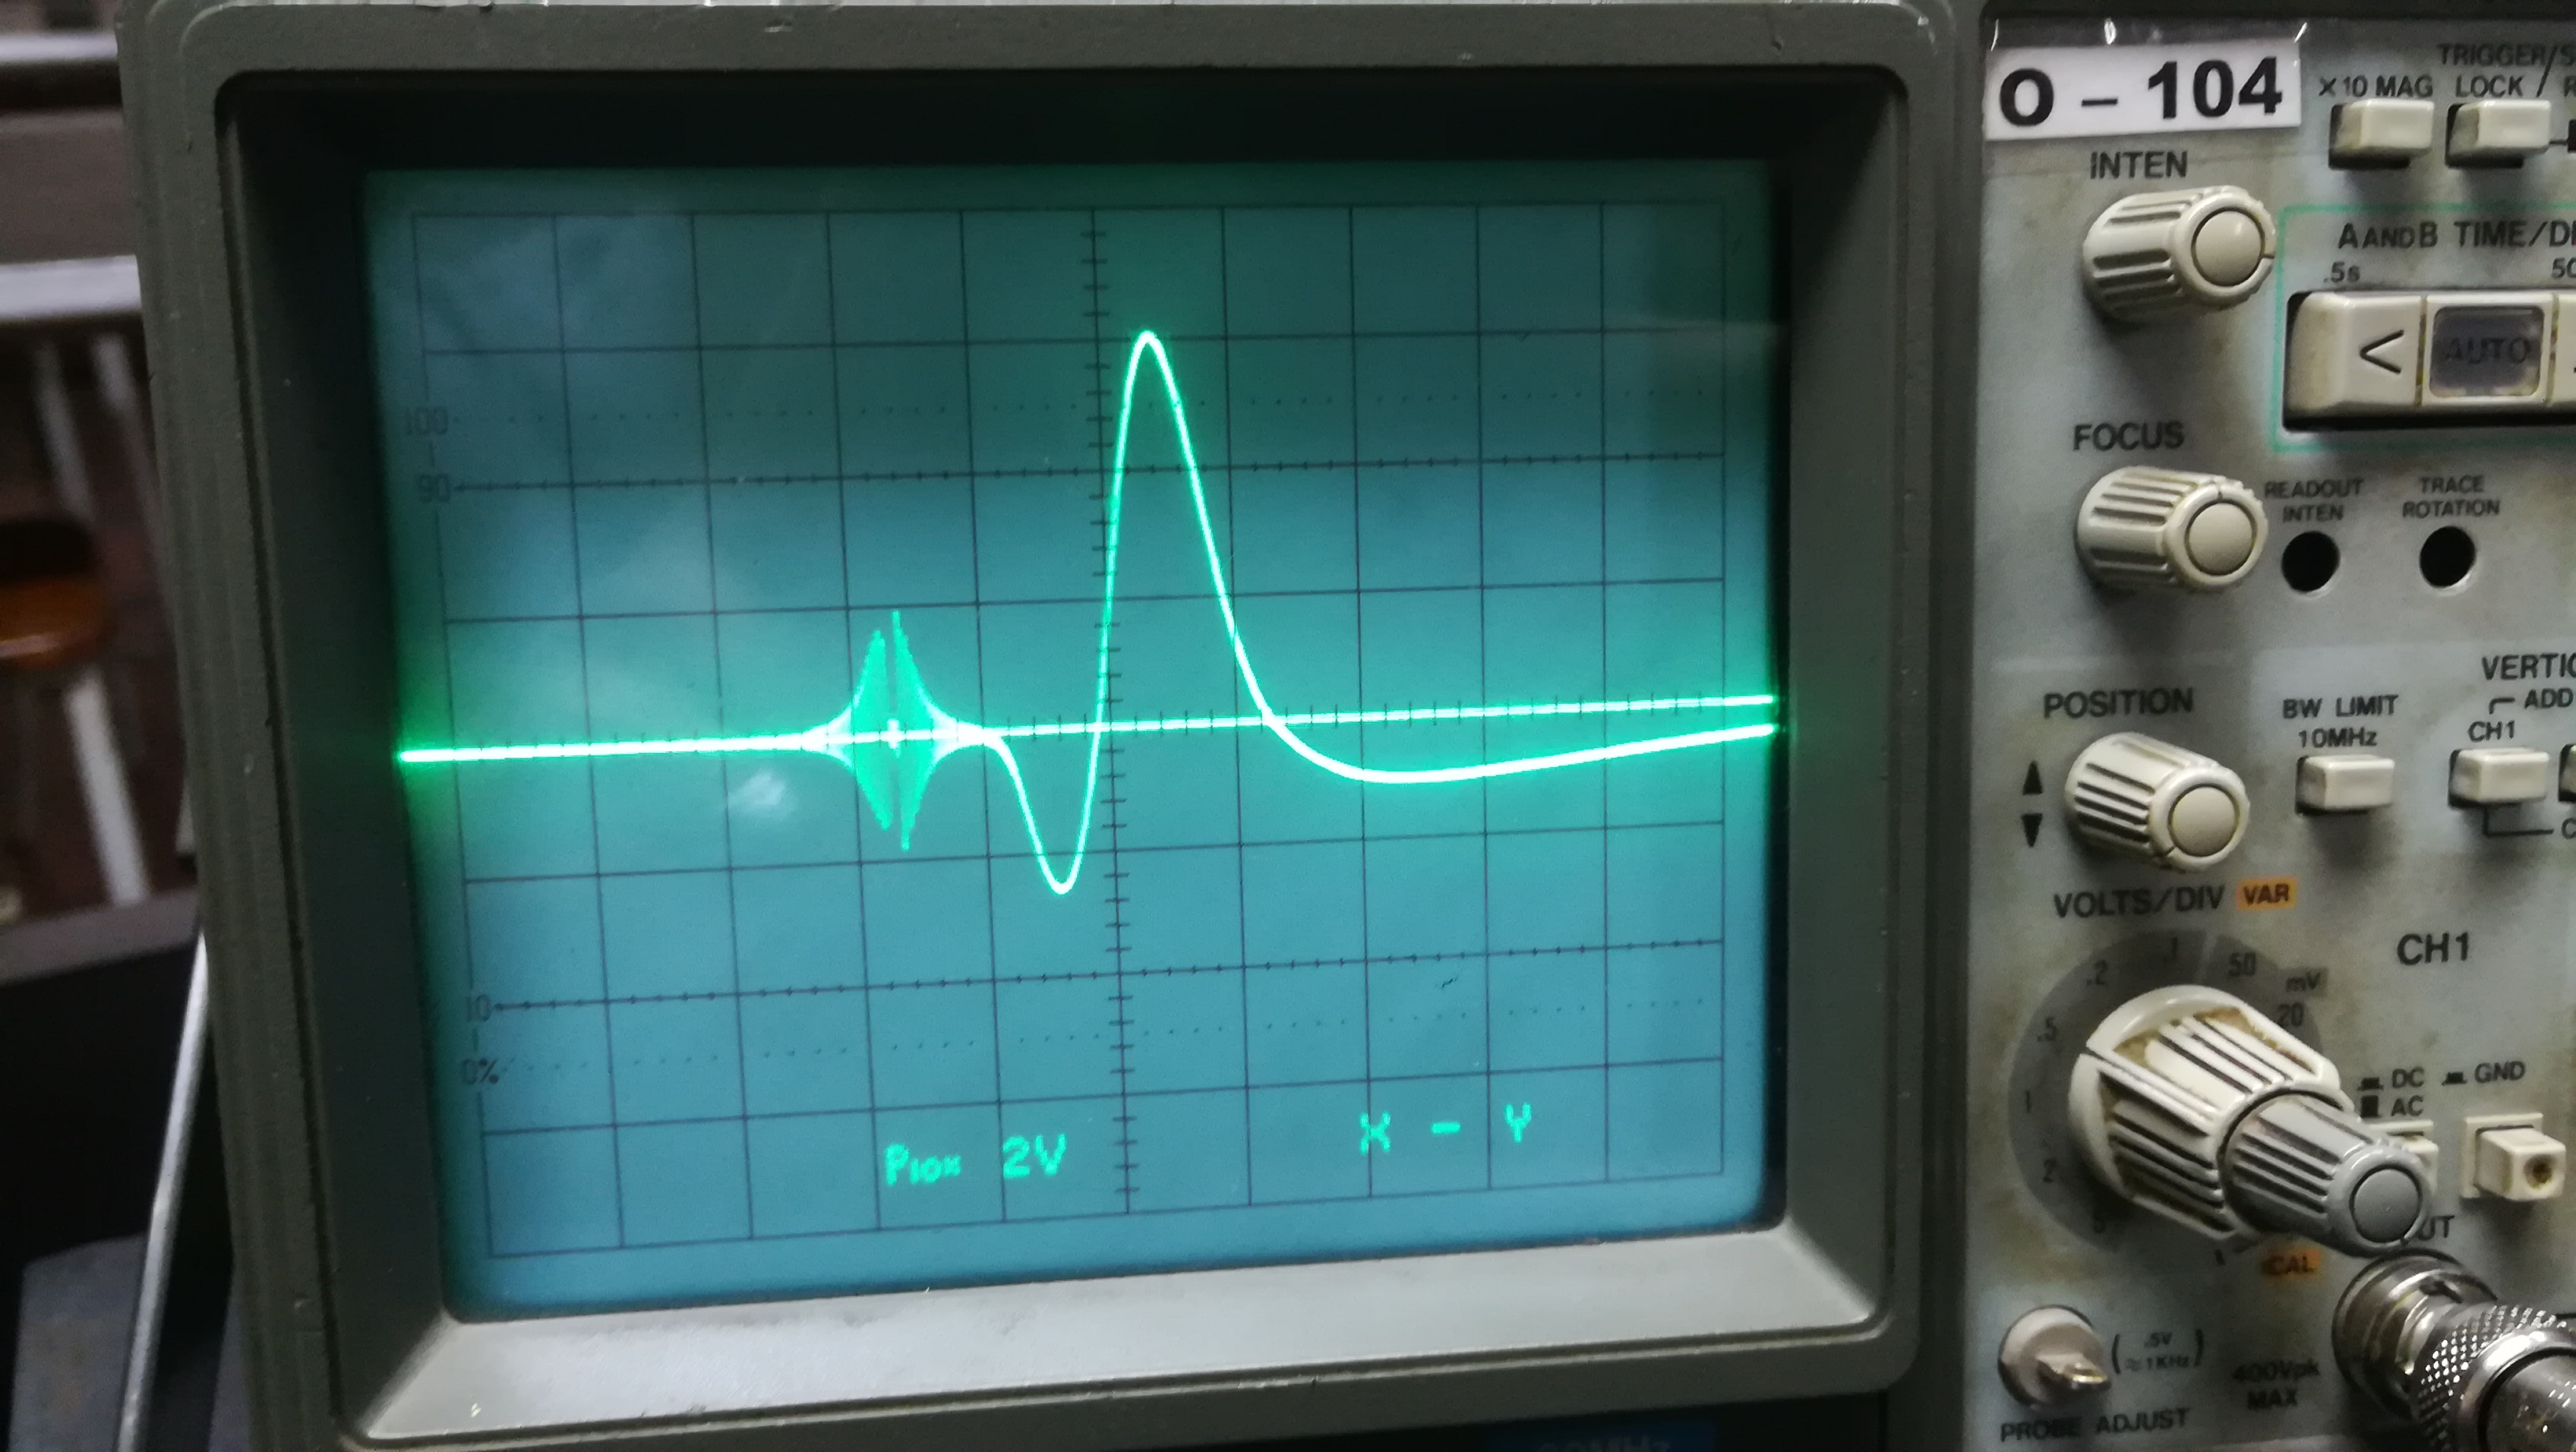
\includegraphics[width=\textwidth]{Imagenes/ActividadPractica/CaracteristicasDeDeteccion/Exp2.2_AmpliFI_MarcaAIzquierda.jpg}}
        \caption{Seteo de la espectro junto con la marca.}
        \label{fig:EspectroaFI}
      \end{subfigure}

      \caption{Espectro del amplificador de FI del detector.}
      \label{fig:MediccionEspectroFIDetector}
    \end{figure}

    Medición de la frecuencia mínima del amplificador de FI y del detector........

    \begin{figure}[H]
      \centering
      \begin{subfigure}[ht]{0.48\textwidth}
        \frame{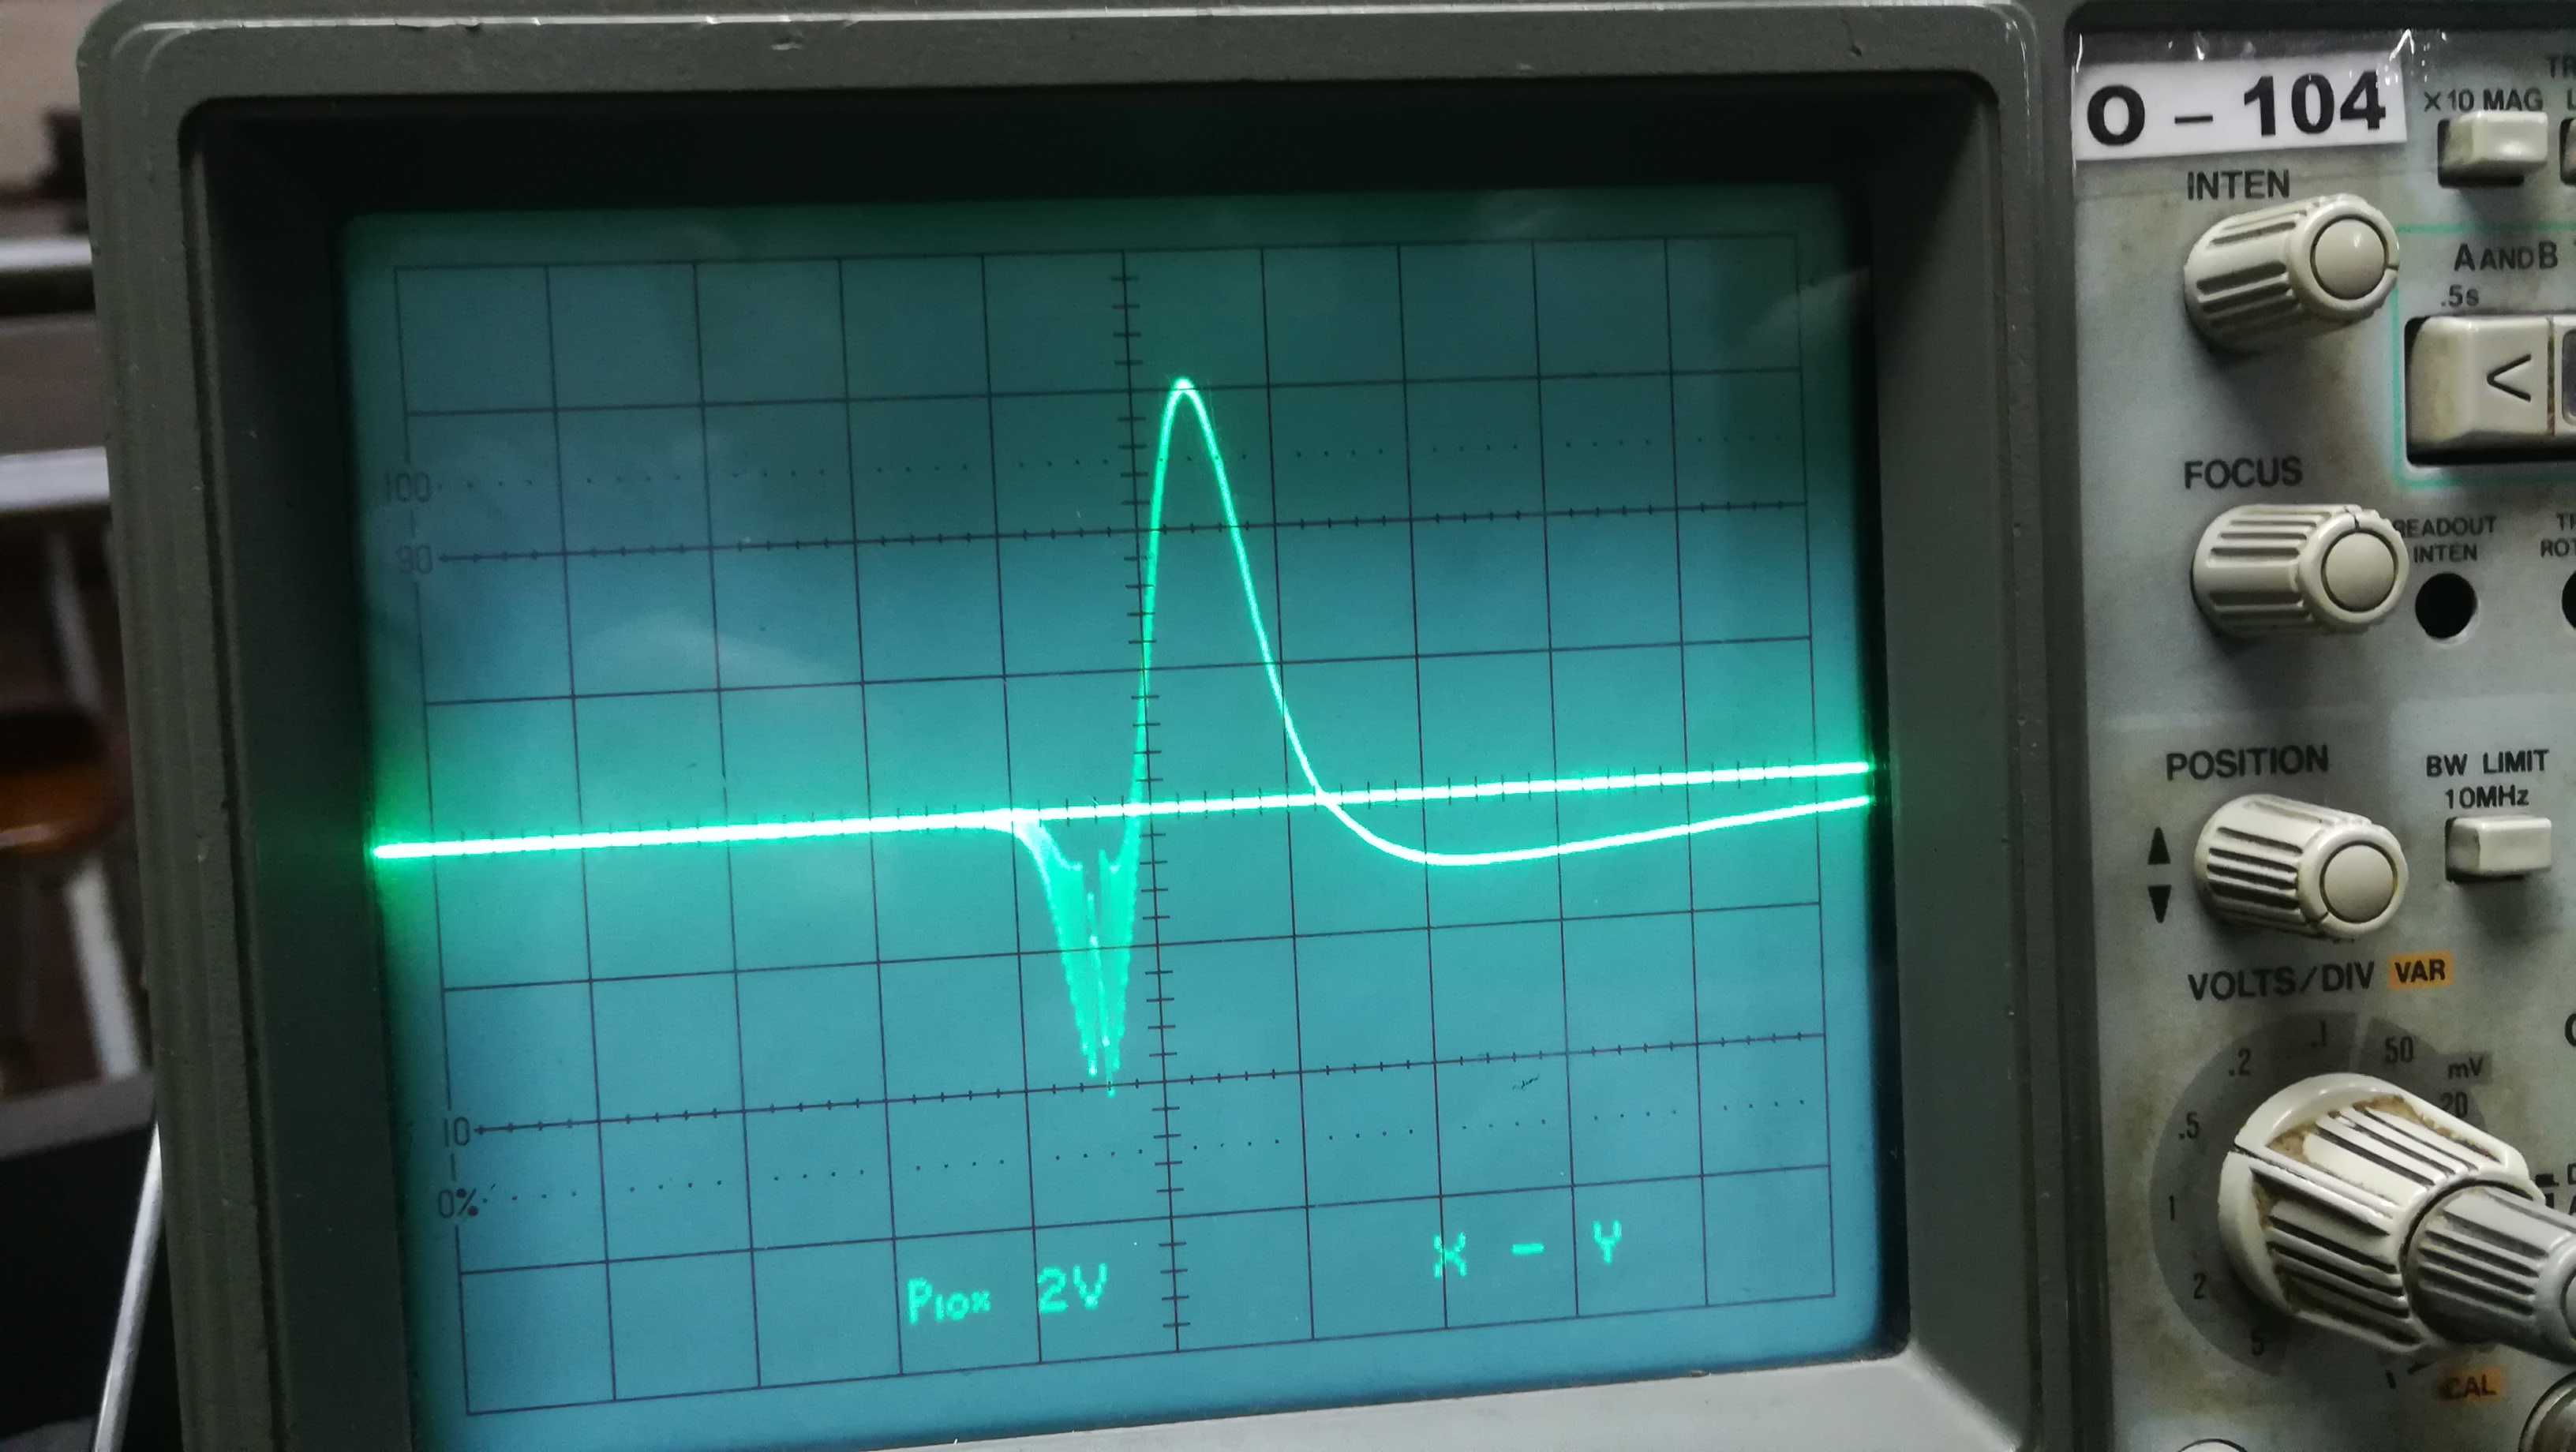
\includegraphics[width=\textwidth]{Imagenes/ActividadPractica/CaracteristicasDeDeteccion/Exp2.4_AmpliFI_FcMin.jpg}}
        \caption{Marca en la frecuencia mínima.}
        \label{fig:FrecuenciaMinFI_Osc}
      \end{subfigure}
      \hfill 
      \begin{subfigure}[ht]{0.48\textwidth}
        \frame{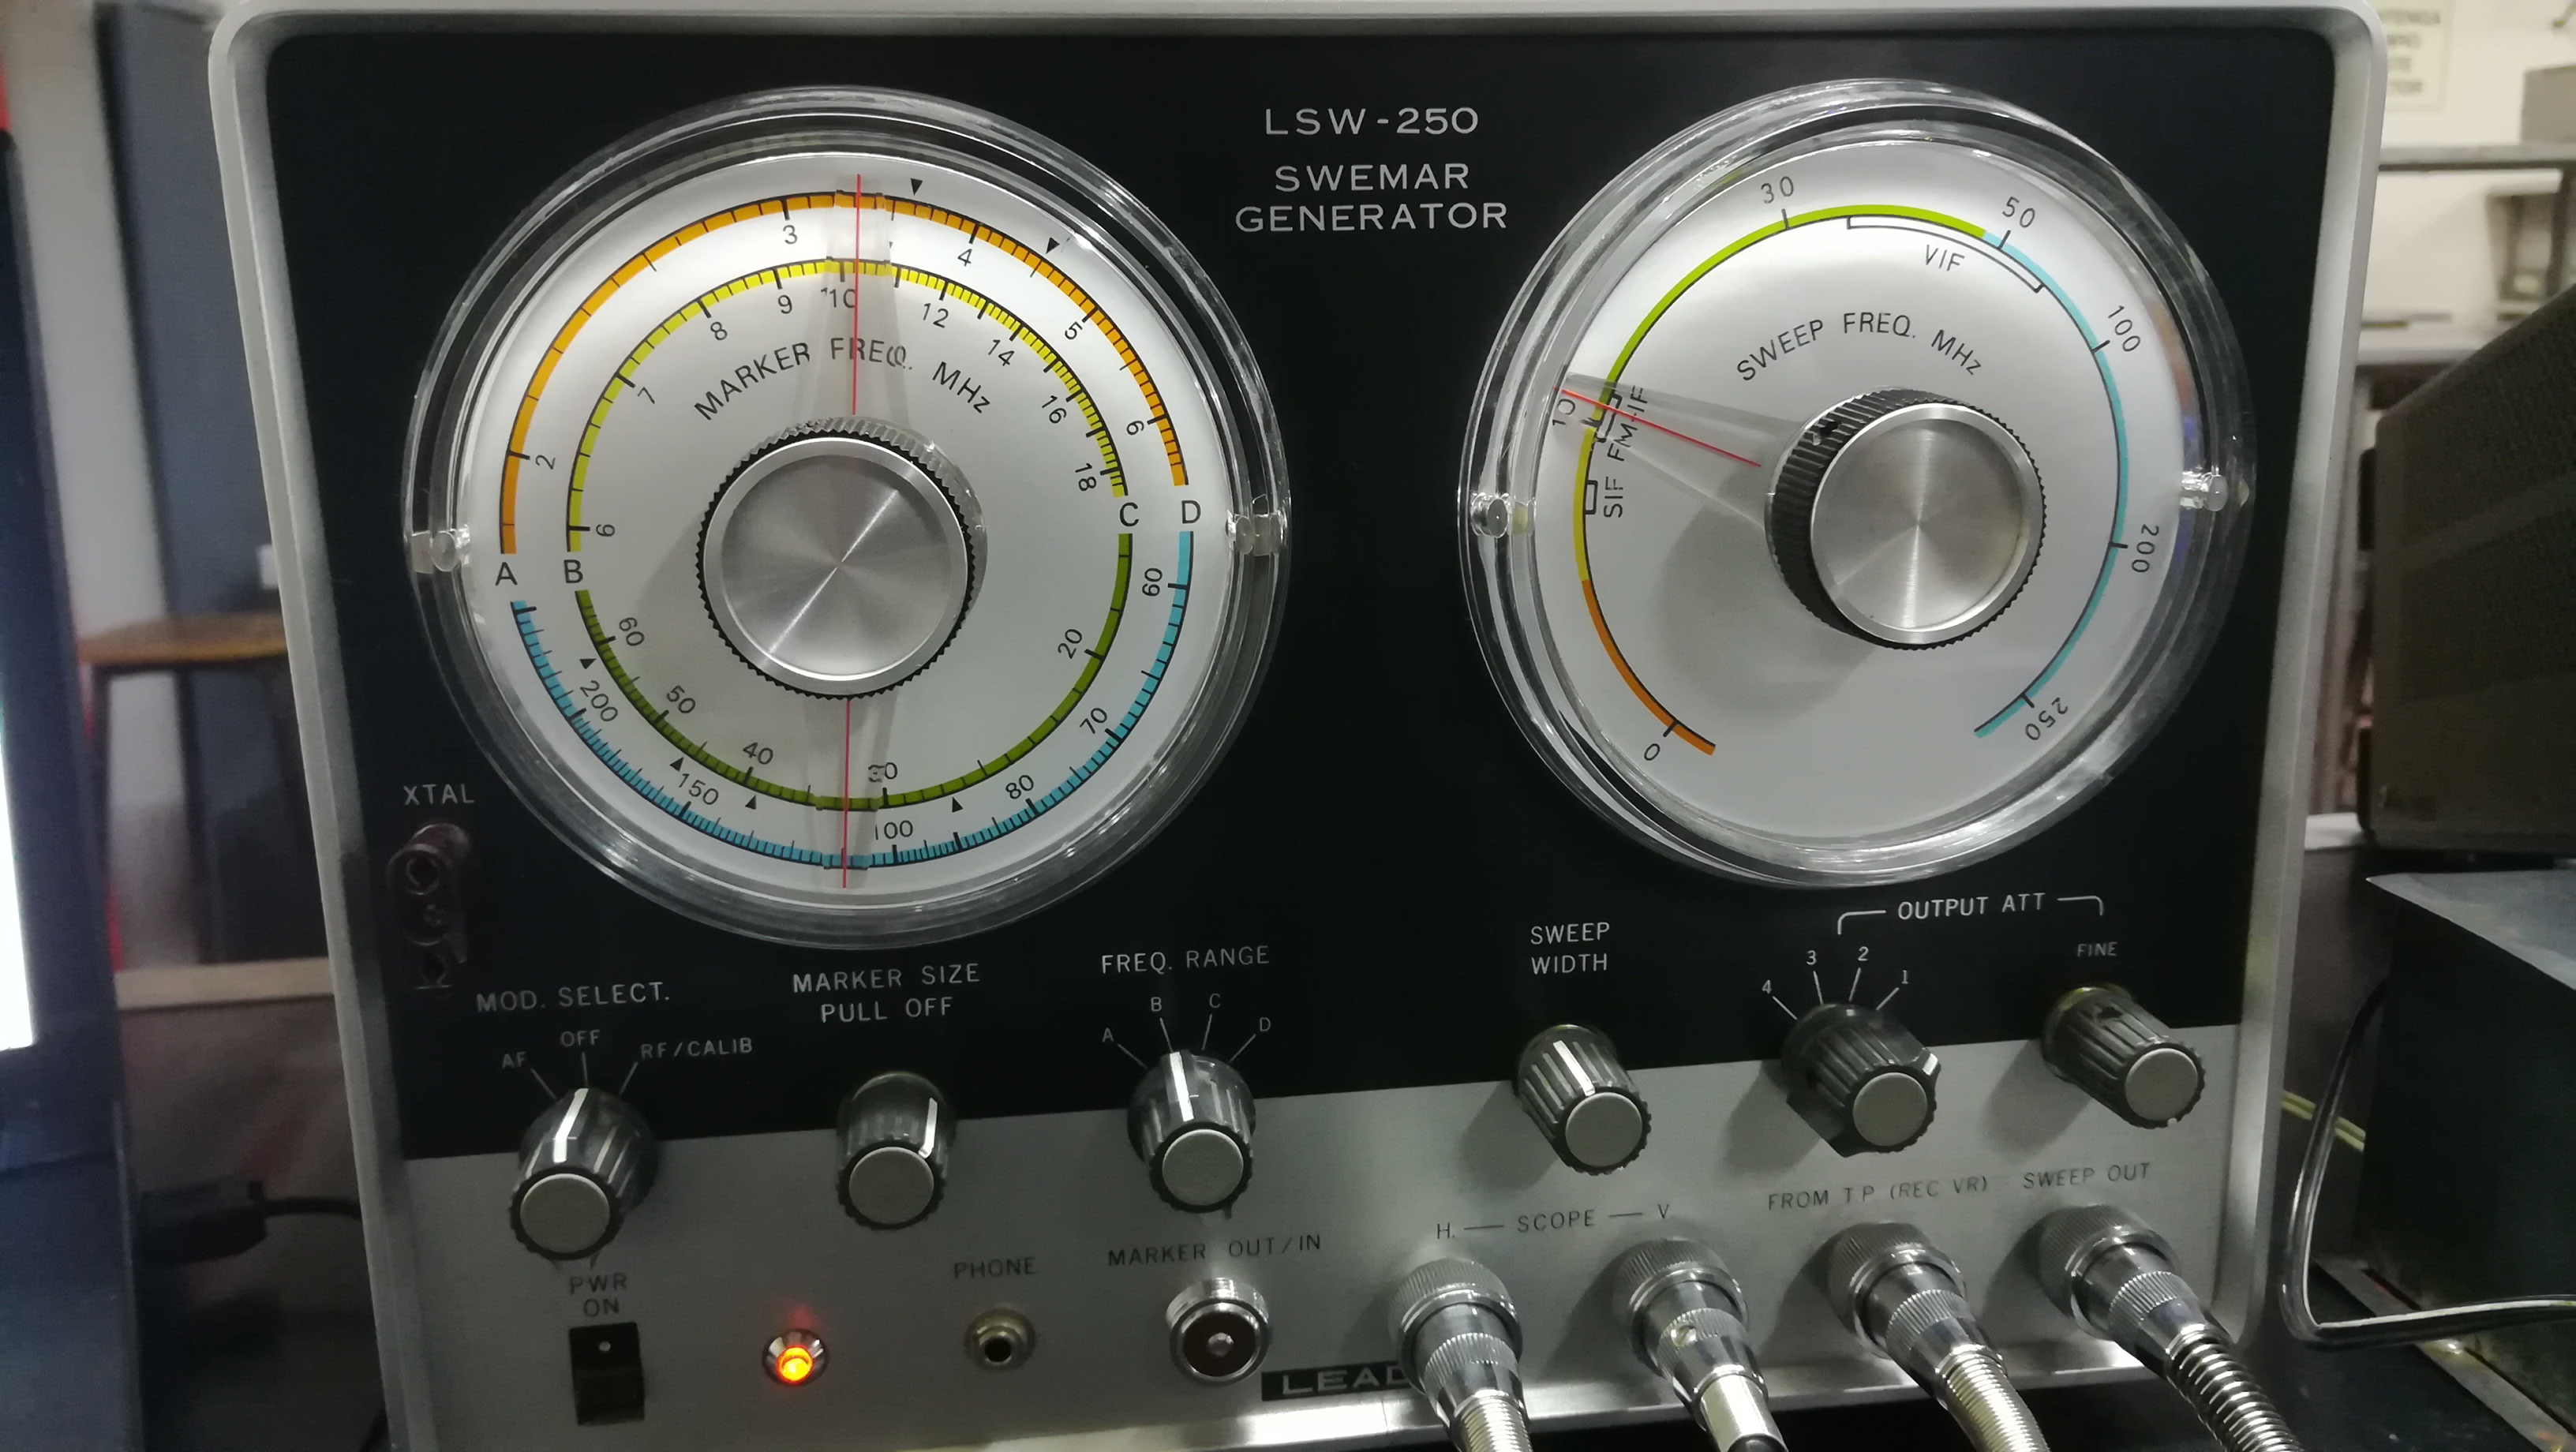
\includegraphics[width=\textwidth]{Imagenes/ActividadPractica/CaracteristicasDeDeteccion/Exp2.5_AmpliFI_FcMin_DialMarca.jpg}}
        \caption{Medición de frecuencia mínima.}
        \label{fig:FrecuneciaMinFI_Gener}
      \end{subfigure}

      \caption{Medición de frecuencia mínima del amplificador de FI y el detector.}
      \label{fig:FrecuenciaMinFI}
    \end{figure}

    Medición de la frecuencia central del amplificador de FI y del detector........

    \begin{figure}[H]
      \centering
      \begin{subfigure}[ht]{0.48\textwidth}
        \frame{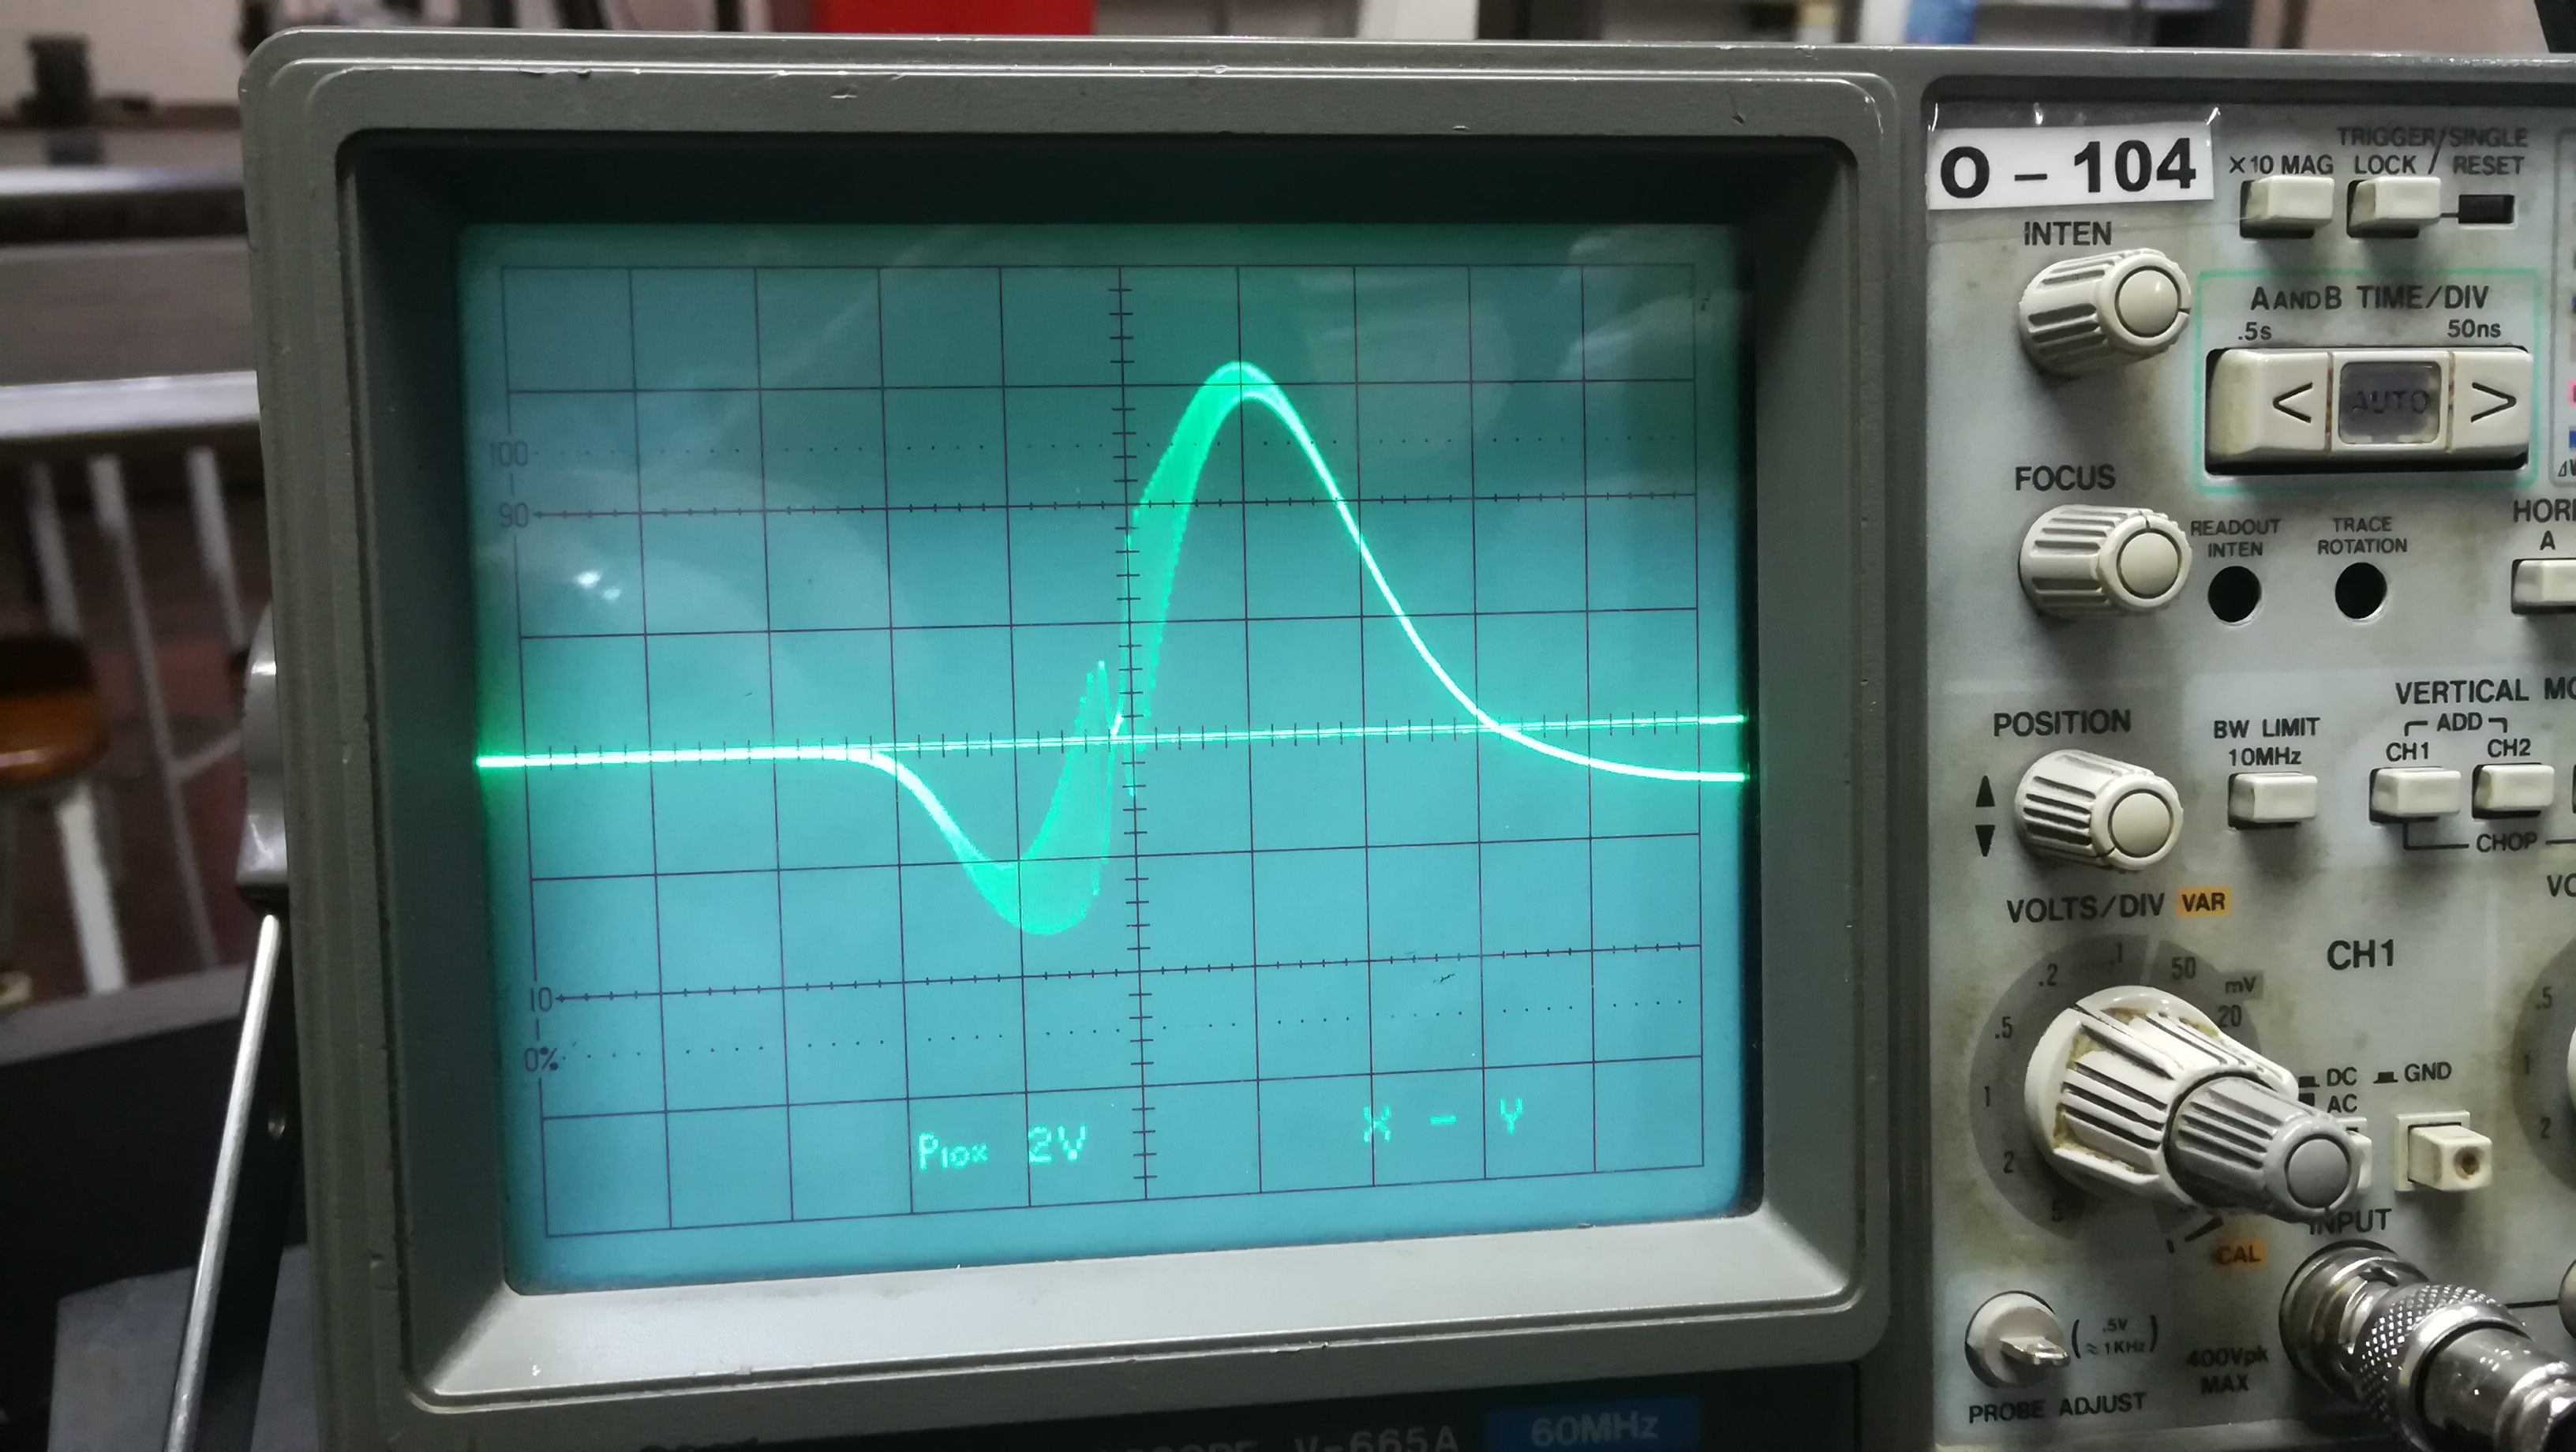
\includegraphics[width=\textwidth]{Imagenes/ActividadPractica/CaracteristicasDeDeteccion/Exp2.9_AmpliFI_FCentral.jpg}}
        \caption{Marca en la frecuencia central.}
        \label{fig:FrecuenciaCenFI_Osc}
      \end{subfigure}
      \hfill 
      \begin{subfigure}[ht]{0.48\textwidth}
        \frame{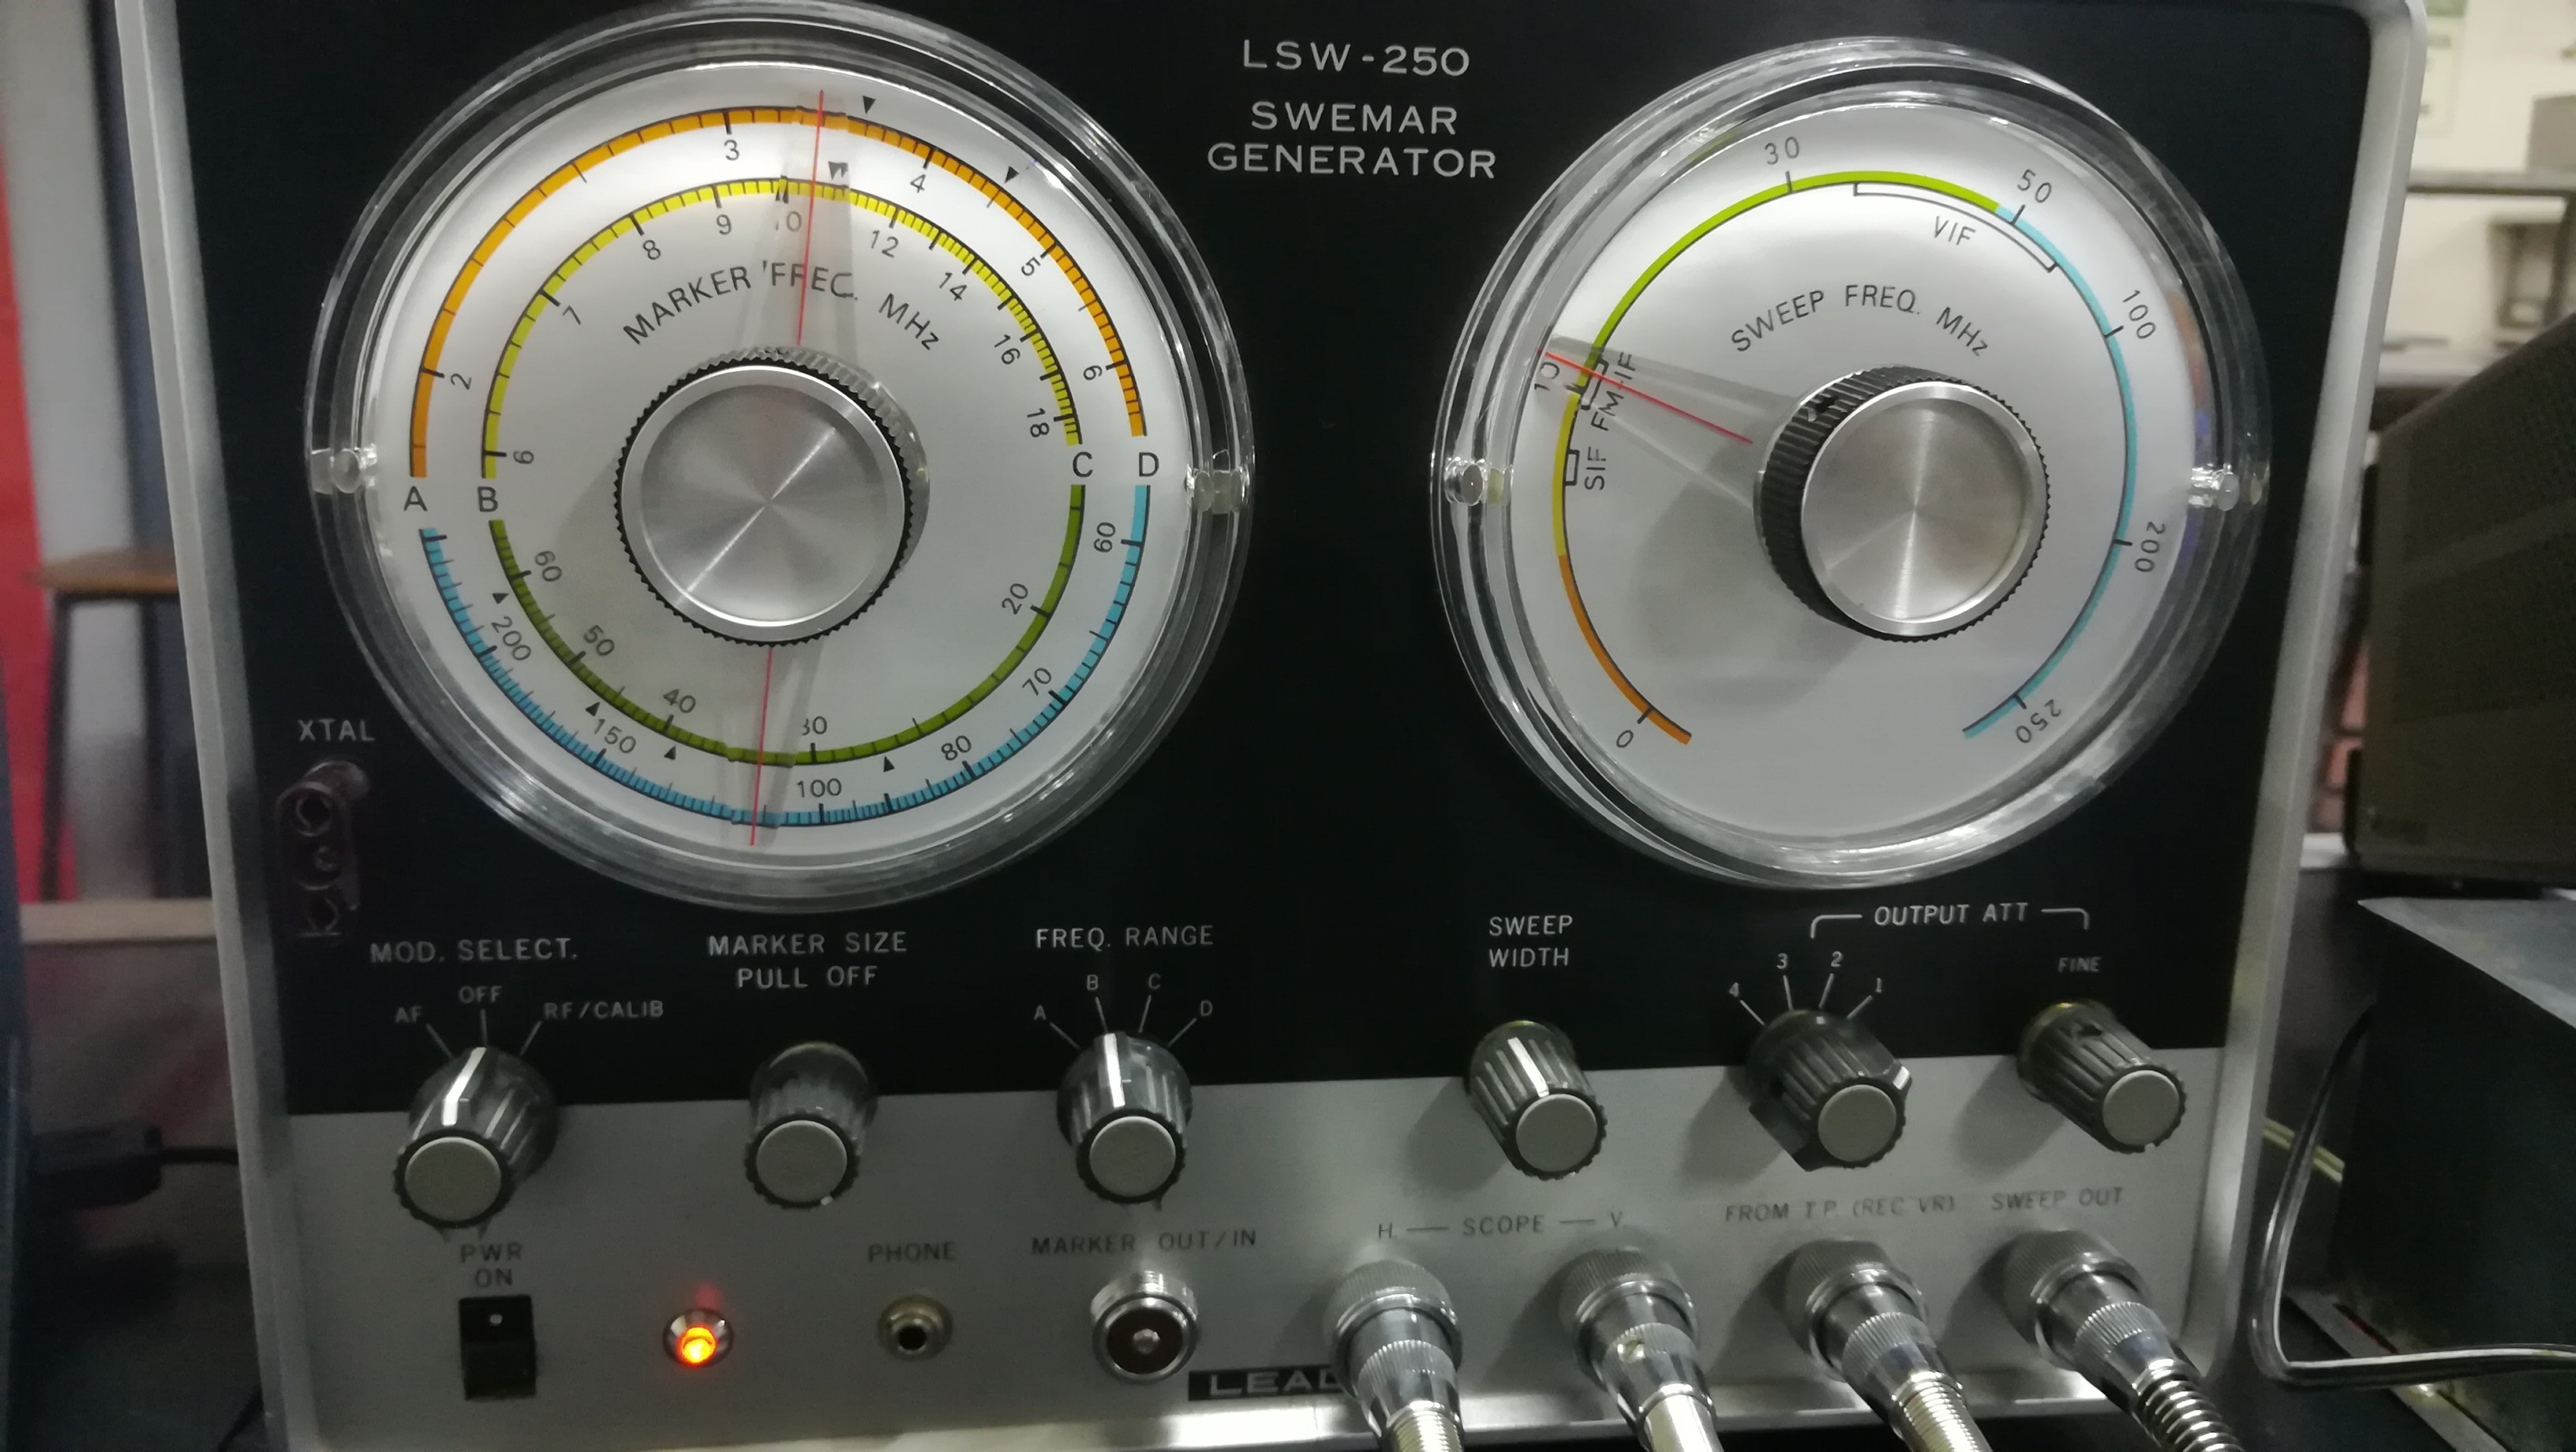
\includegraphics[width=\textwidth]{Imagenes/ActividadPractica/CaracteristicasDeDeteccion/Exp2.9_AmpliFI_FCentral_DialMarca.jpg}}
        \caption{Medición de frecuencia central.}
        \label{fig:FrecuneciaCenFI_Gener}
      \end{subfigure}

      \caption{Medición de frecuencia central del amplificador de FI y el detector.}
      \label{fig:FrecuenciaCenFI}
    \end{figure}

    Medición de la frecuencia máxima del amplificador de FI y del detector........

    \begin{figure}[H]
      \centering
      \begin{subfigure}[ht]{0.48\textwidth}
        \frame{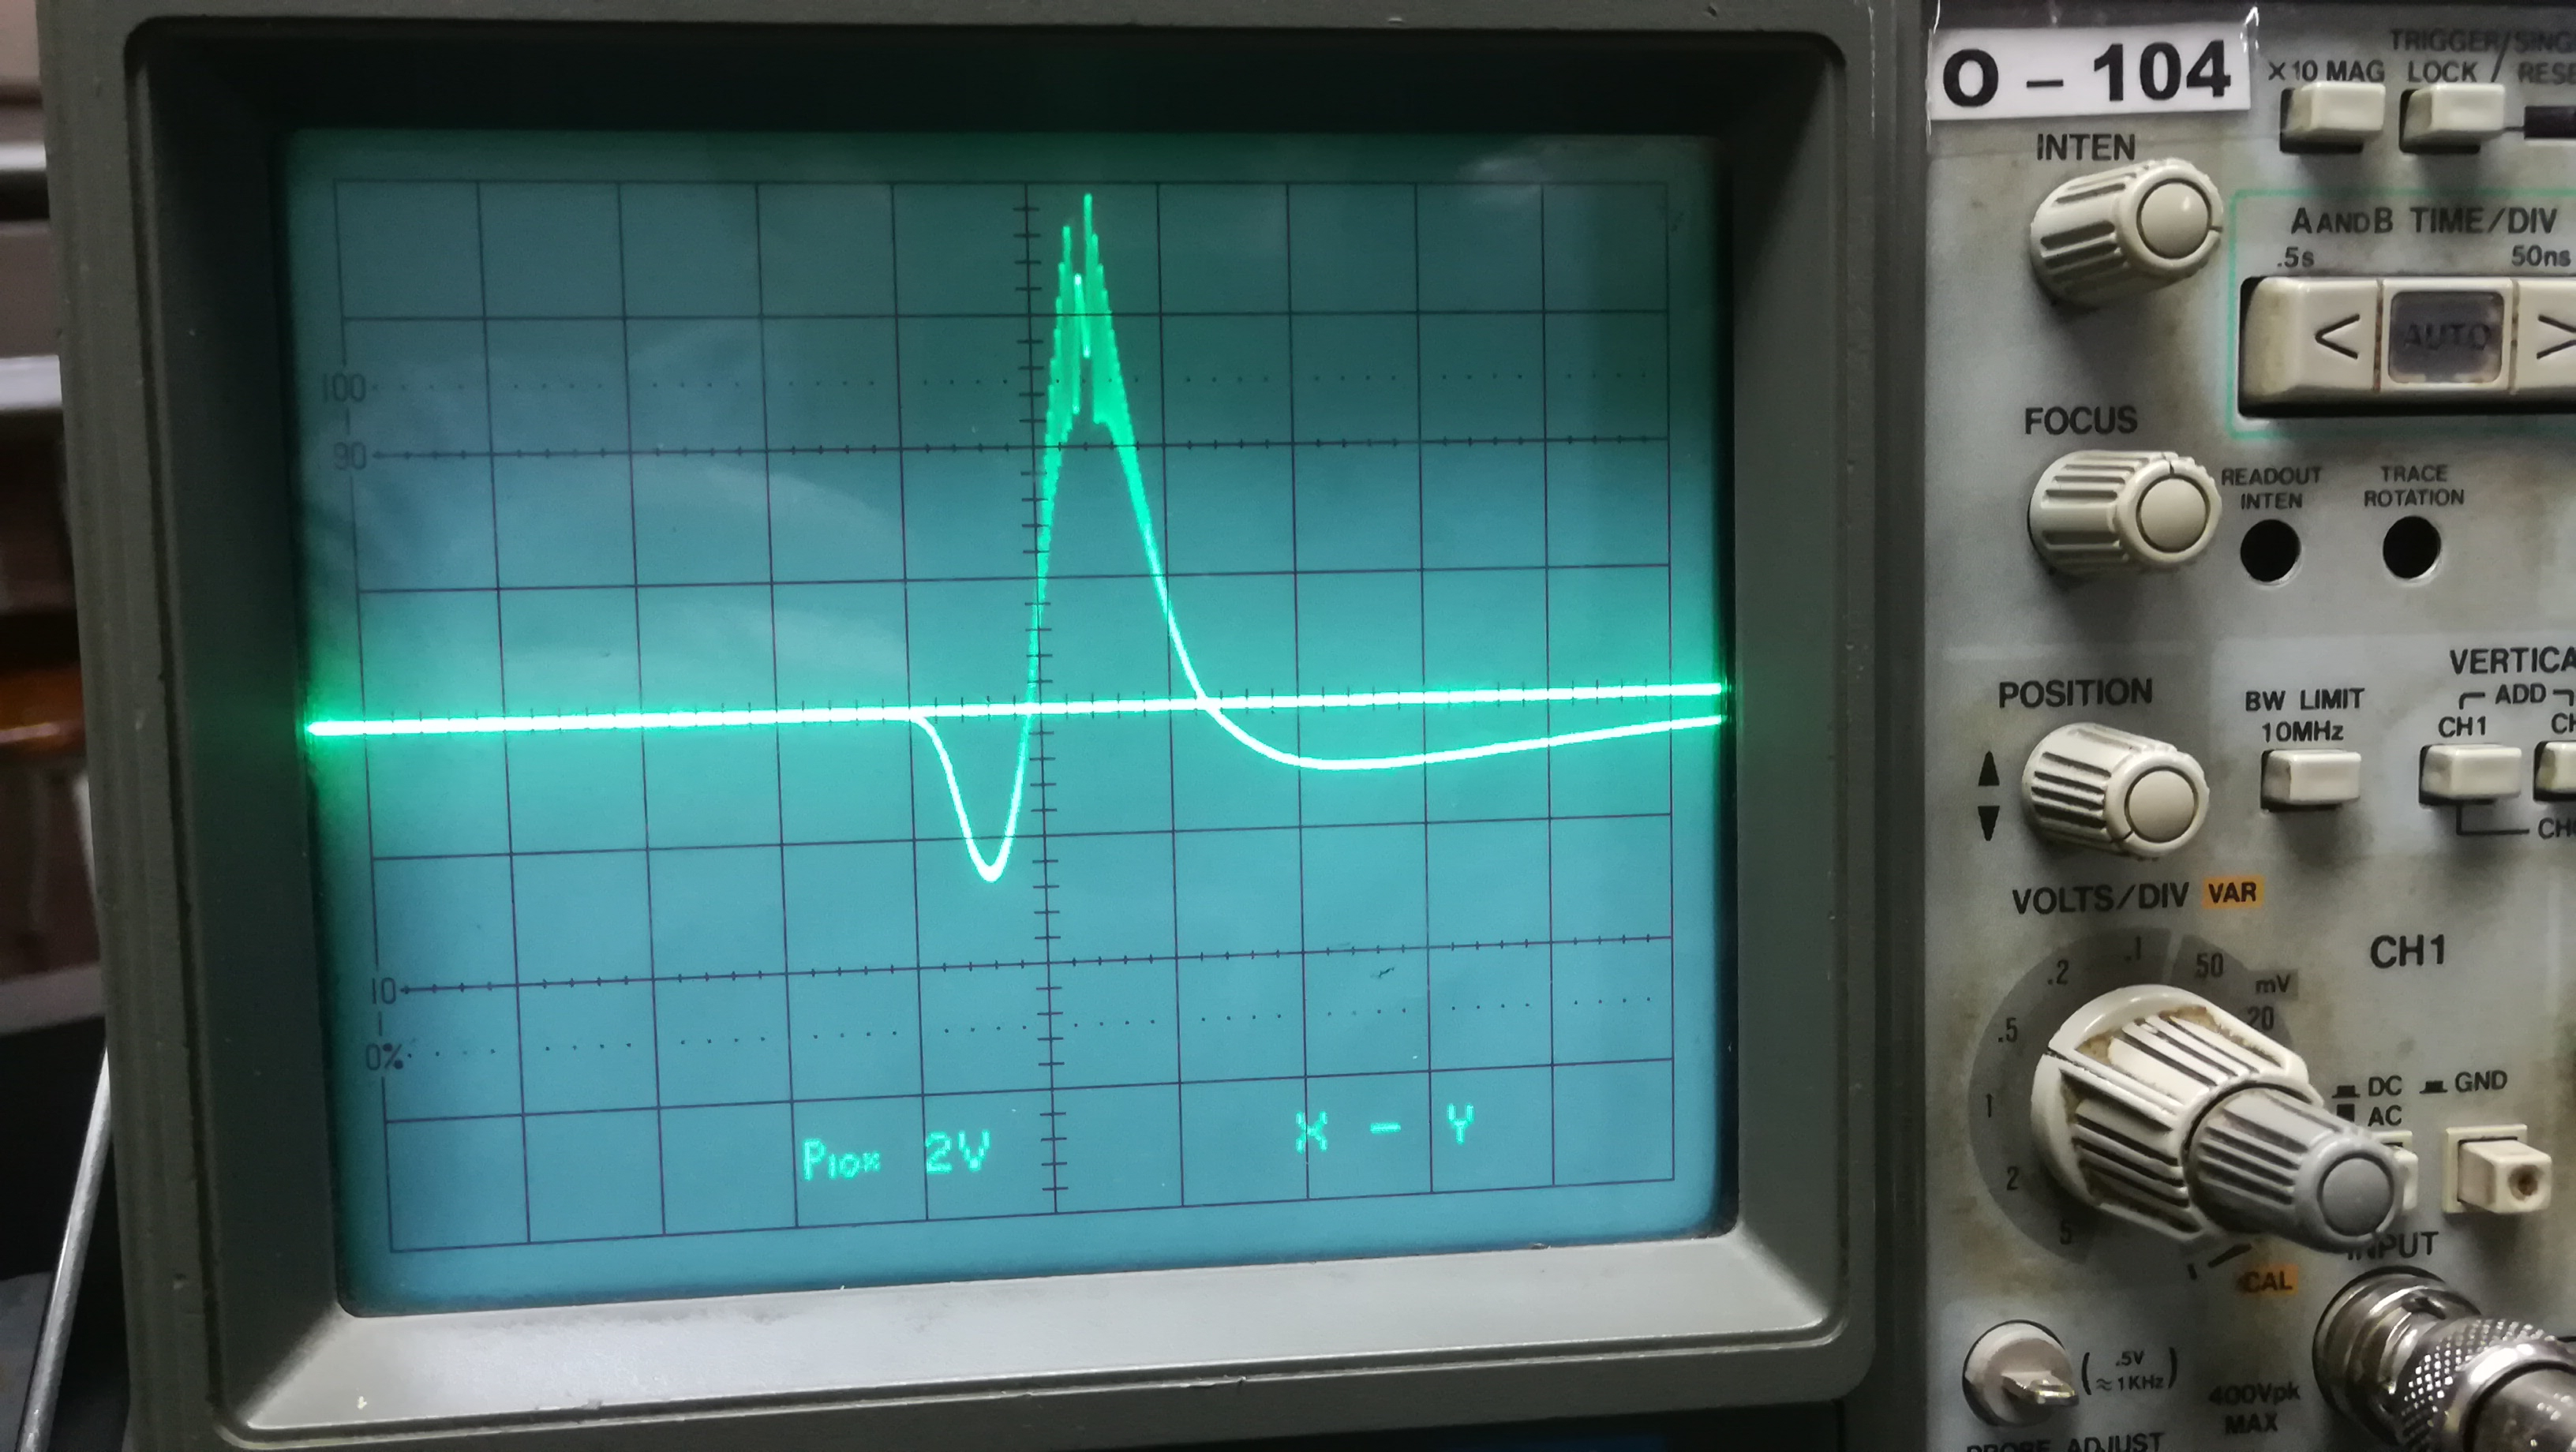
\includegraphics[width=\textwidth]{Imagenes/ActividadPractica/CaracteristicasDeDeteccion/Exp2.6_AmpliFI_FcMax.jpg}}
        \caption{Marca en la frecuencia máxima.}
        \label{fig:FrecuenciaMaxFI_Osc}
      \end{subfigure}
      \hfill 
      \begin{subfigure}[ht]{0.48\textwidth}
        \frame{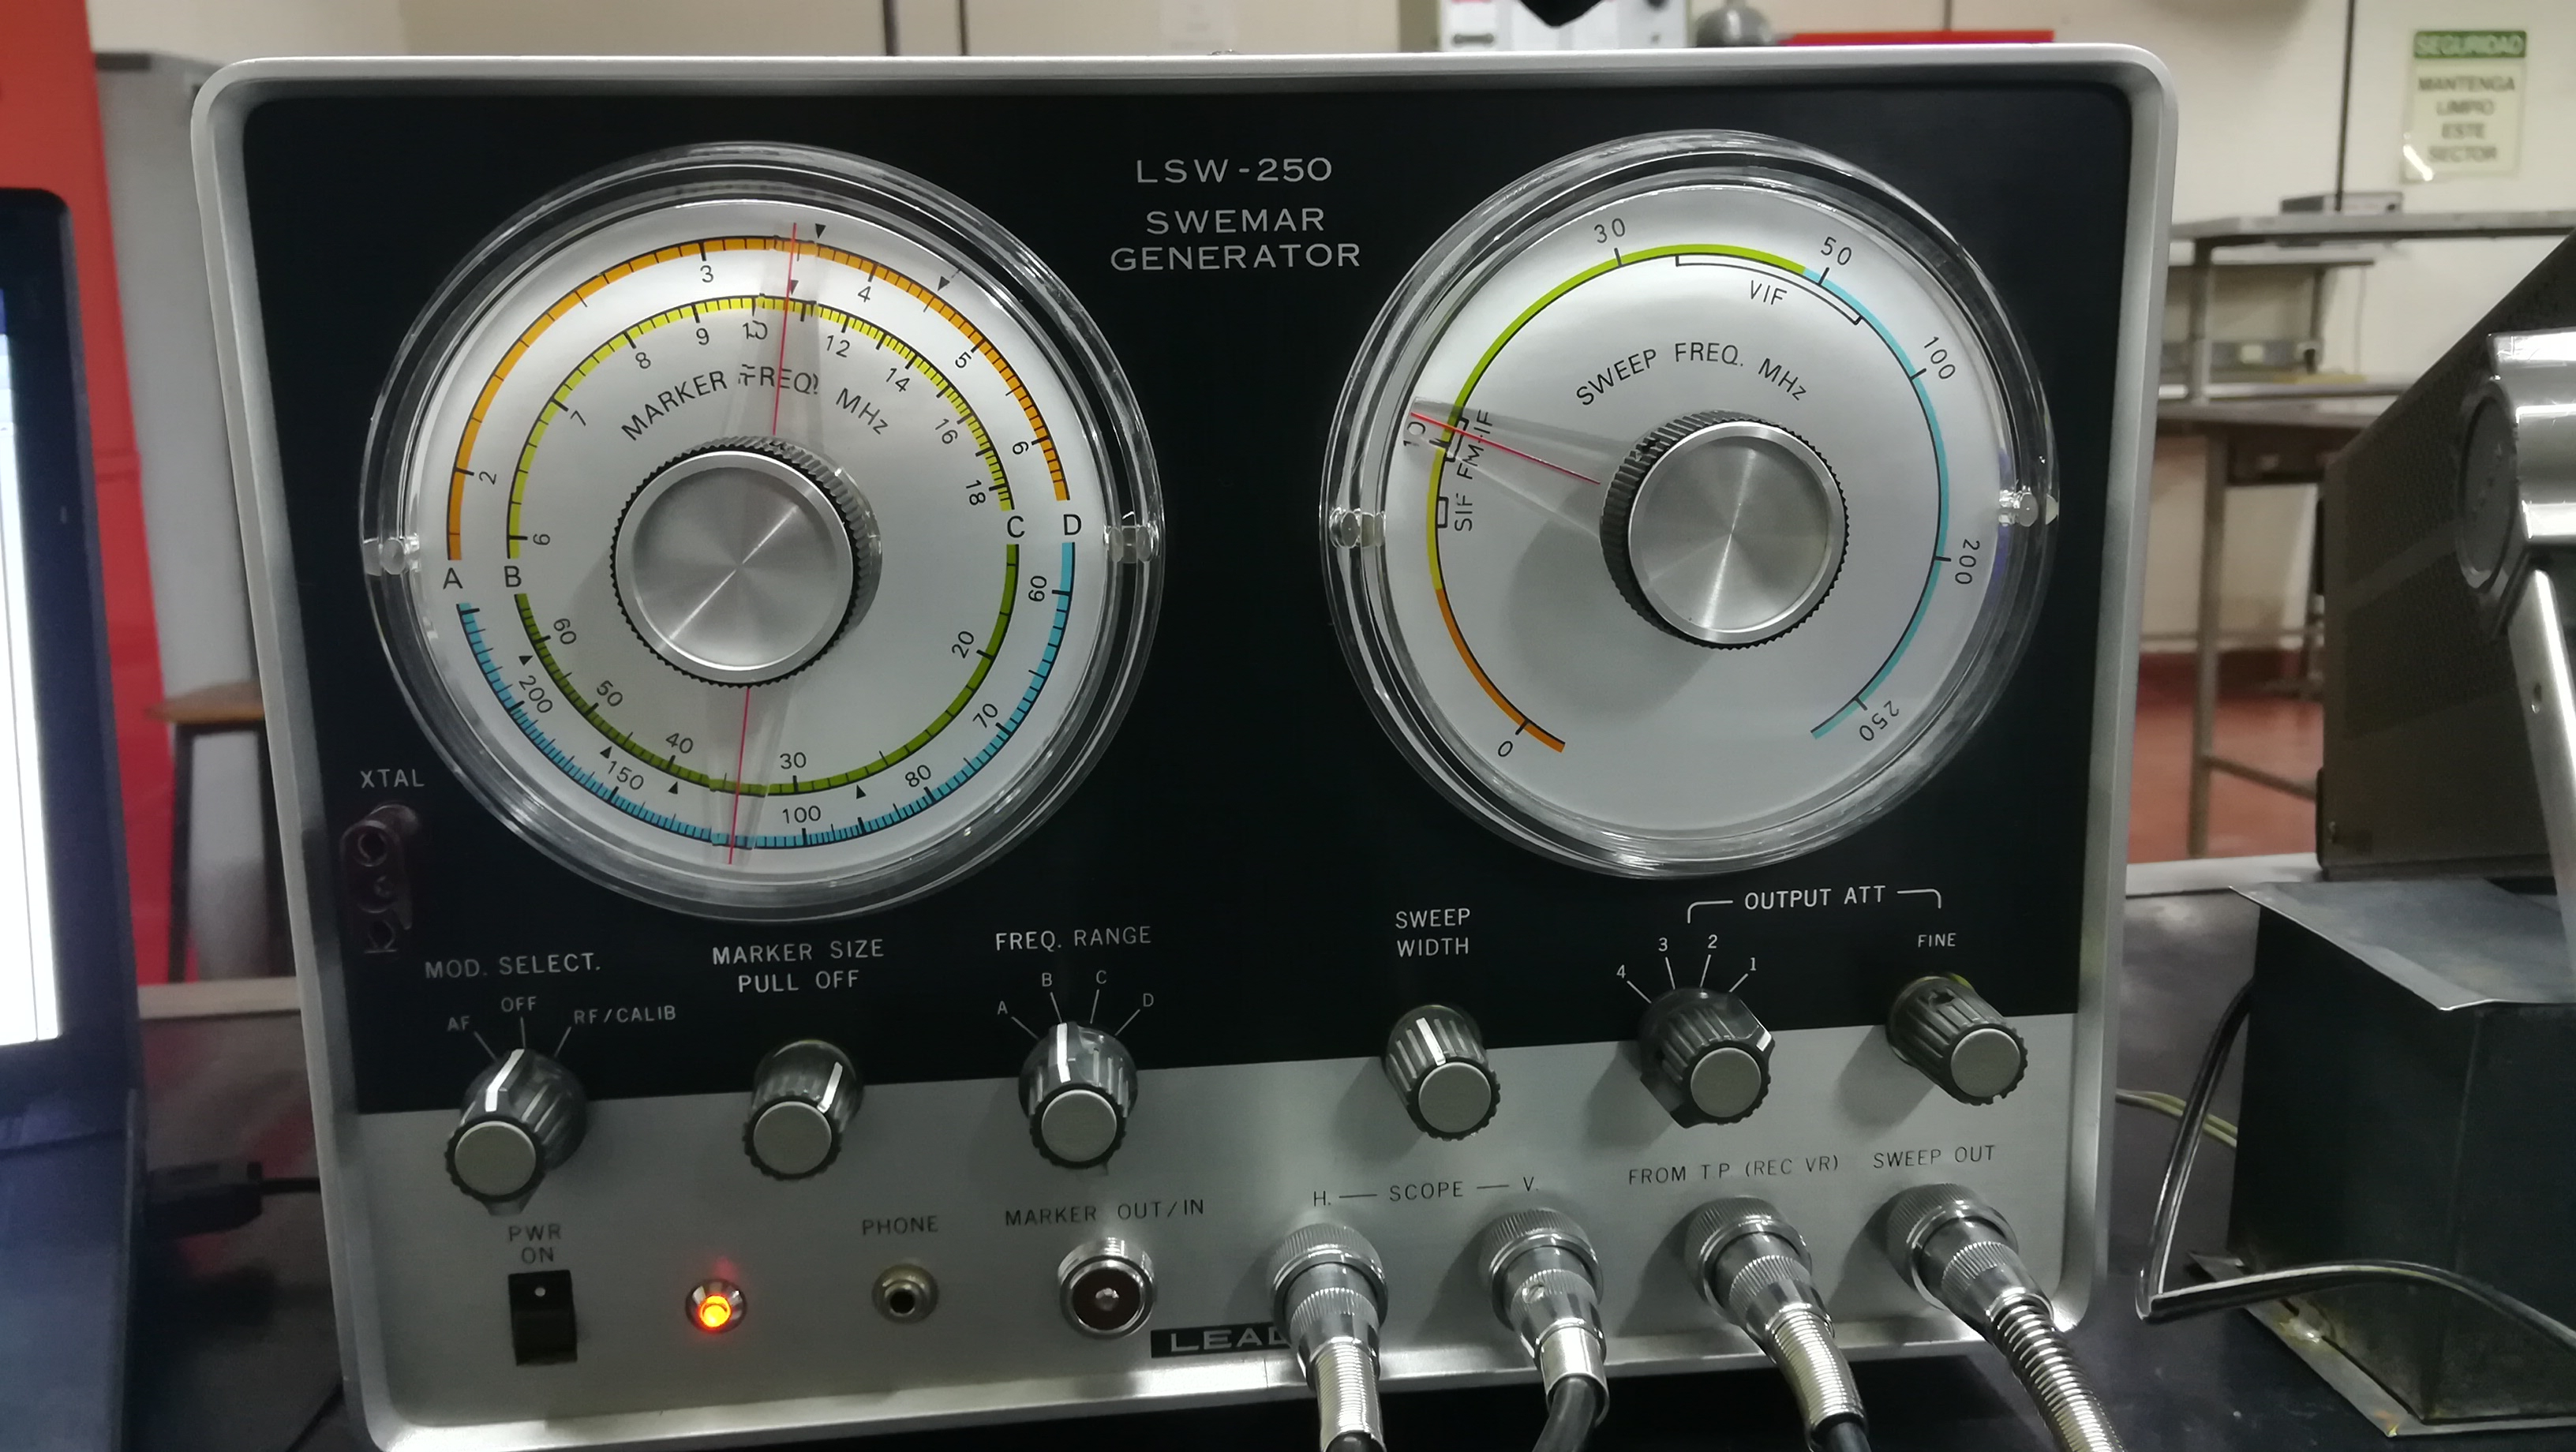
\includegraphics[width=\textwidth]{Imagenes/ActividadPractica/CaracteristicasDeDeteccion/Exp2.7_AmpliFI_FcMax_DialMarca.jpg}}
        \caption{Medición de frecuencia máxima.}
        \label{fig:FrecuneciaMaxFI_Gener}
      \end{subfigure}

      \caption{Medición de frecuencia máxima del amplificador de FI y el detector.}
      \label{fig:FrecuenciaMaxFI}
    \end{figure}

